\section{ハード構成}\label{ux5168ux4f53ux69cbux6211}

ハード構成、および電気回路は第3章と同じで、Fig.\ref{fig401}になります。

\begin{figure}[htbp]
    \centering
    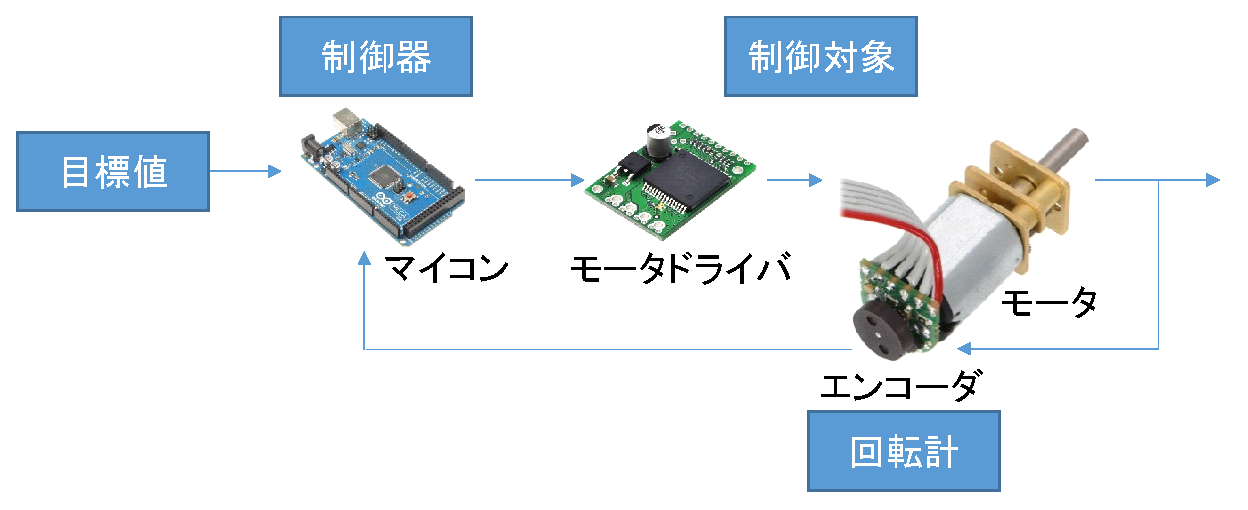
\includegraphics[width=300pt]{fig/fig401.eps}
    \caption{ハード構成}
    \label{fig401}
\end{figure}


\section{PID制御モデル}\label{ux6a5fux4f53ux306eux72b6ux614bux3068ux30b5ux30a4ux30ba}

SimulinkによるPID制御モデルはFig.\ref{fig402}の通りです。
PID Controller ブロックのパラメータはFig.\ref{fig403}の値を入力しました。
Saturation ブロックのパラメータはFig.\ref{fig404}の値を入力しました。
今回のモータはDC6Vで29000~30000rpmにて回るので、
Saturation1 ブロックにはモータ最大回転数より若干低い値を入力します。
Saturation2 ブロックには操作量の上下限で飽和するようにします。

\begin{figure}[htbp]
    \centering
    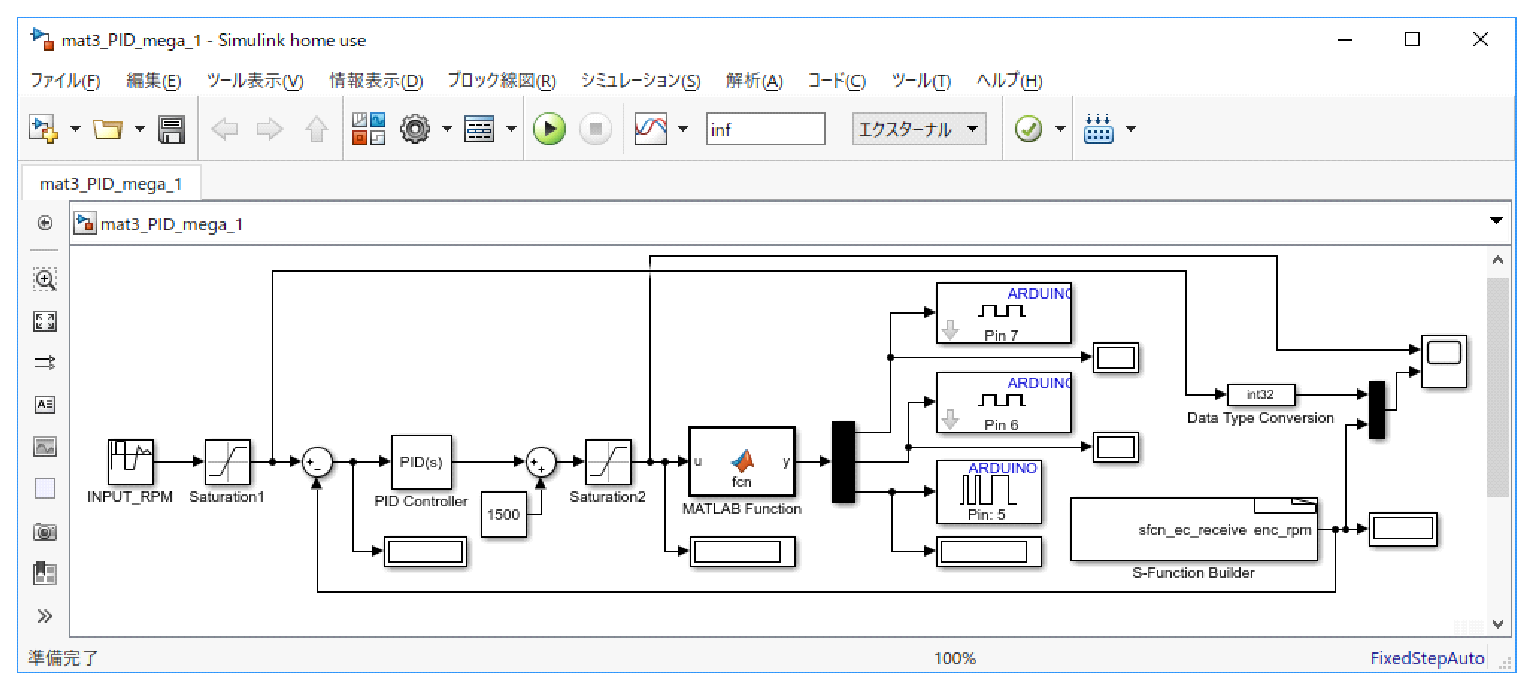
\includegraphics[width=389pt]{fig/fig402.eps}
    \caption{PID制御のSimulinkモデル}
    \label{fig402}
\end{figure}

\begin{figure}[htbp]
    \centering
    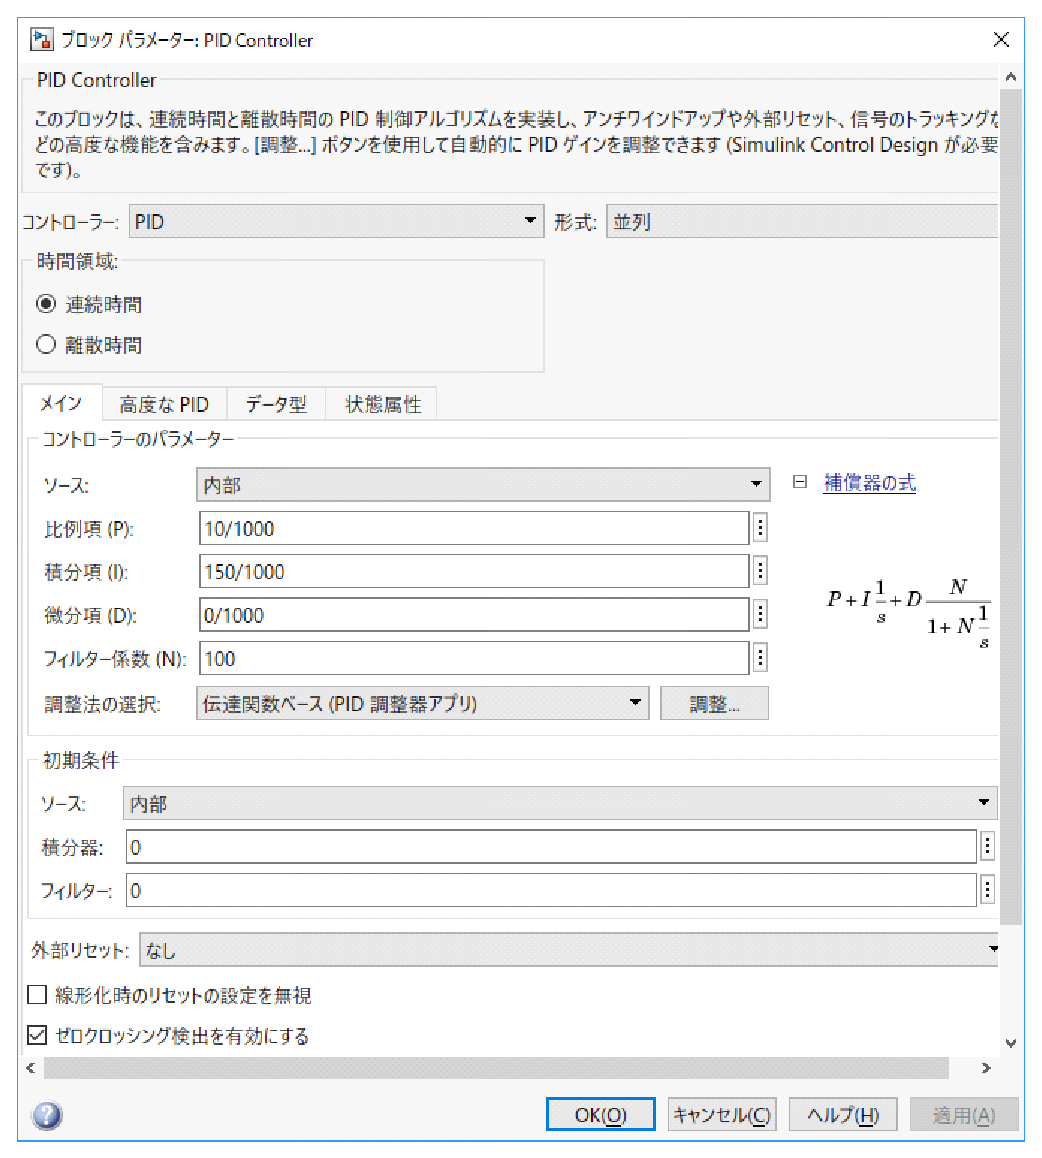
\includegraphics[width=250pt]{fig/fig403.eps}
    \caption{PID Controller ブロック パラメータ}
    \label{fig403}
\end{figure}

\begin{figure}[htbp]
    \centering
    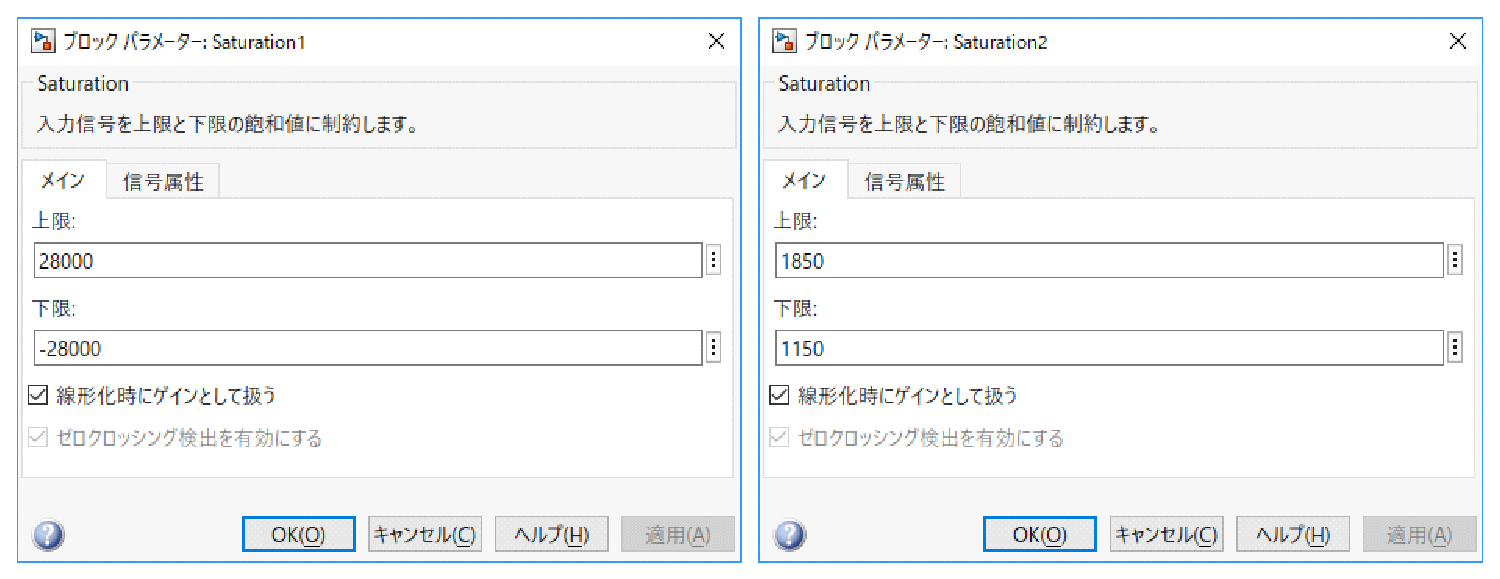
\includegraphics[width=350pt]{fig/fig404.eps}
    \caption{Saturation ブロック パラメータ}
    \label{fig404}
\end{figure}


%\clearpage
\section{実行}\label{ux30a2ux30fcux30e0ux69cbux6210ux306eux8a73ux7d30}

回転数の計測結果をFig.\ref{fig405}に示します。
回転数の黄色線が目標の回転数で、青線が実測値になります。
目標に対して実測値がおおむね追従していることが確認できます。

\begin{figure}[htbp]
    \centering
    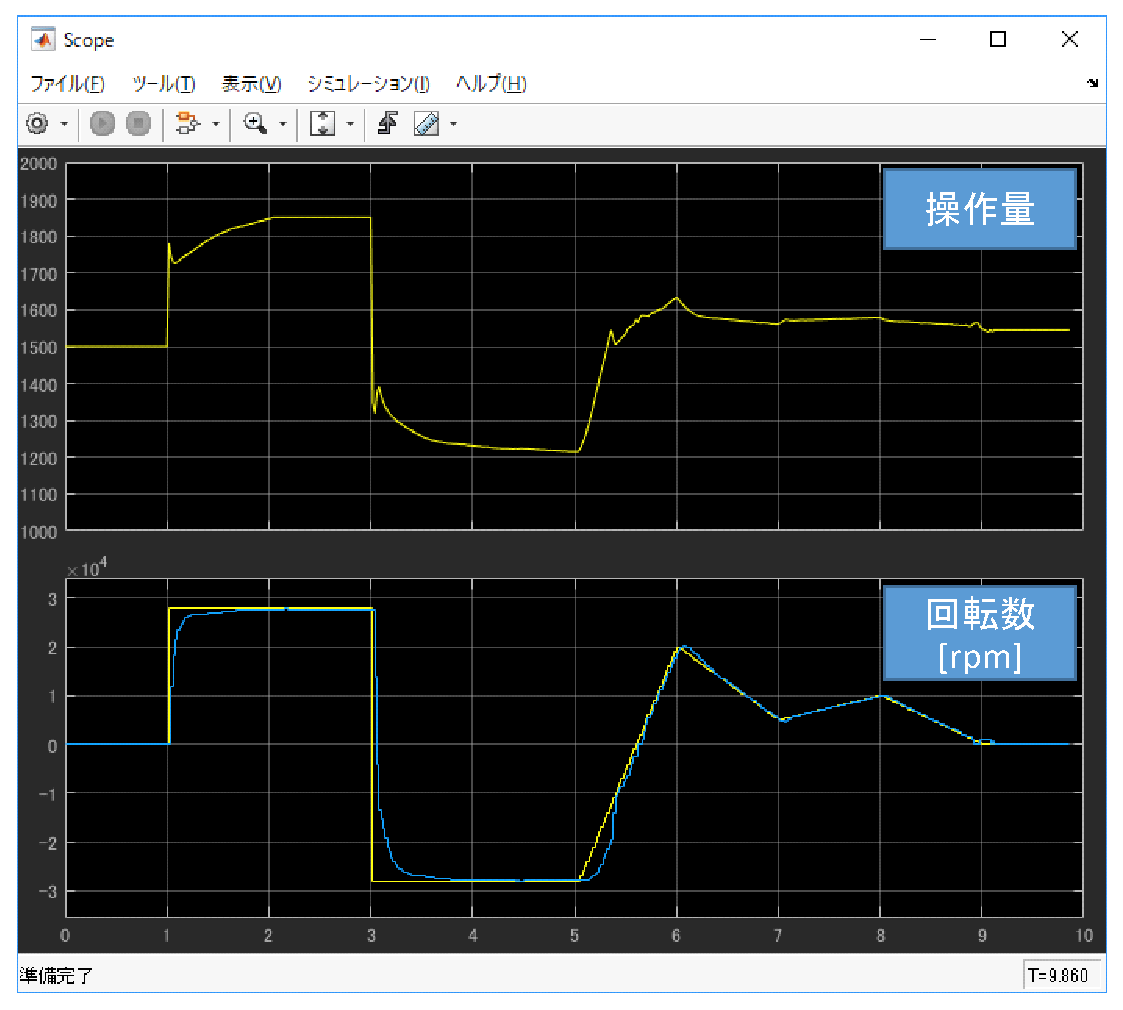
\includegraphics[width=200pt]{fig/fig405.eps}
    \caption{回転数の計測結果}
    \label{fig405}
\end{figure}


\section{ロボットへの実装例}\label{ux7a4dux5c64ux65b9ux5411ux306eux5272ux308cux9632ux6b62ux69cbux6210}

Fig.\ref{fig101}に示したロボットへの実装例になります。
本ロボットは脚ユニットを4脚使用しています。
そのハード構成はFig.\ref{fig406}の通りです。
中央制御基板で受信機からのラジコン信号を読み取り、
I2C通信で各脚制御基板に回転数目標値を出力しています。

Fig.\ref{fig407}に中央制御基板のSimulinkモデルを示します。
ラジコン信号の読み取り方法は
Using an RC Controller with Arduino and Simulink\cite{MathWors_RC_receive}
を参考にしました。
読み取ったラジコン信号のバルス幅をローパスフィルタにかけ、
パルス幅から回転数目標に変換し、
I2Cブロックに入力するため、回転数目標値を+-の符号を含め3byteのデータに変換しています。

Fig.\ref{fig408}に脚制御基板のSimulinkモデルを示します。
I2C通信をS-function ブロックで実現する方法は
ADLX345 i2c Driver for Arduino Mega\cite{MathWors_I2C}
を参考にしました。
I2C Masterから読み取った回転数目標値は、3byteデータを復号して
Fig.\ref{fig402}で作製したモデルの入力側に接続しています。

実行例をFig.\ref{fig409}に示します。
手で操作したプロポの挙動に応じて、回転数を制御することができます。

\begin{figure}[htbp]
    \centering
    \includegraphics[width=350pt]{fig/fig406.eps}
    \caption{ロボットへの実装}
    \label{fig406}
\end{figure}

\begin{figure}[htbp]
    \centering
    \includegraphics[width=389pt]{fig/fig407.eps}
    \caption{中央制御基板のSimulinkモデル (I2C Master)}
    \label{fig407}
\end{figure}

\begin{figure}[htbp]
    \centering
    \includegraphics[width=389pt]{fig/fig408.eps}
    \caption{脚制御基板のSimulinkモデル (I2C Slave)}
    \label{fig408}
\end{figure}

\begin{figure}[htbp]
    \centering
    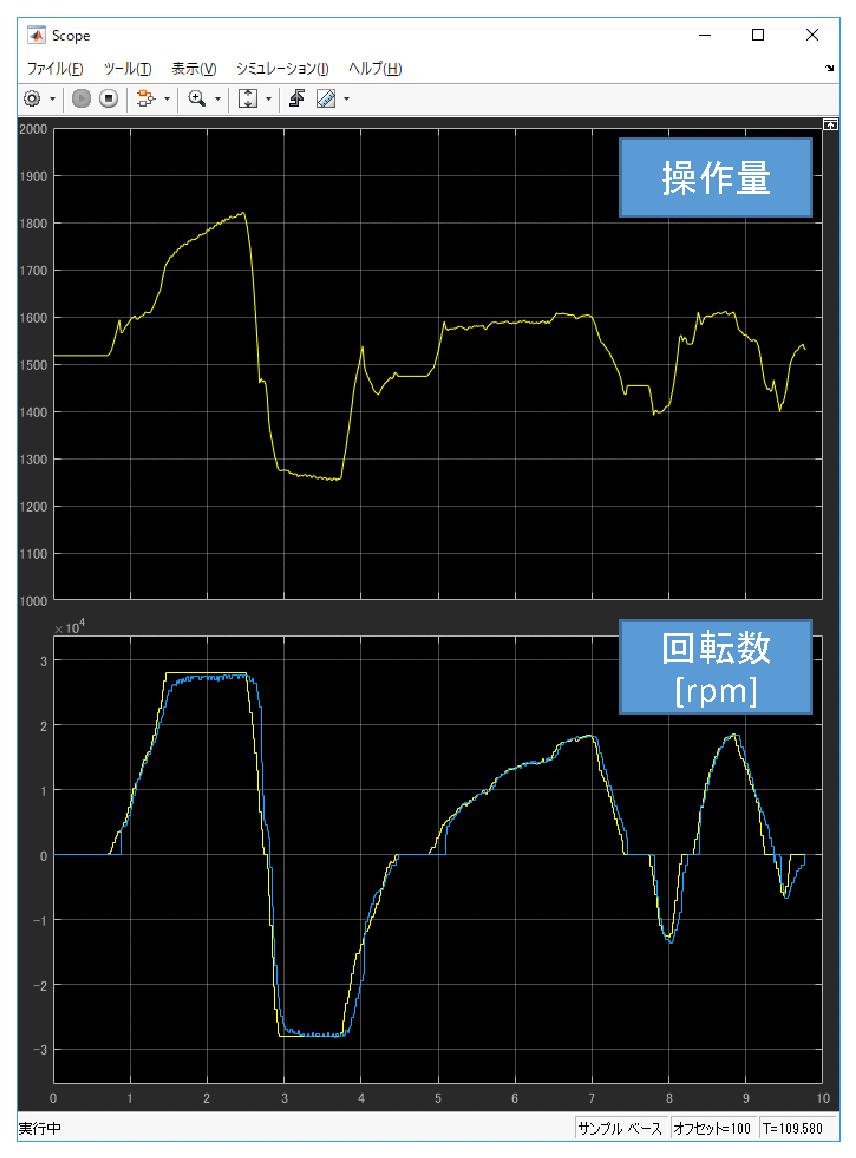
\includegraphics[width=200pt]{fig/fig409.eps}
    \caption{実行例}
    \label{fig409}
\end{figure}

